
\section{Quiz Bowl: A Game of Human Coreference}
\label{sec:qb-data}

One example of such data comes from a game called \emph{quiz bowl}.  Quiz bowl
is a trivia game where questions are structured as a series of sentences, all of
which indirectly refer to the answer. Each question has multiple clusters of
mutually-coreferent terms, and one of those clusters is coreferent with the
answer. Figure~\ref{fig:qbexample} shows an example of a quiz bowl question
where all answer coreferences have been marked.

\begin{figure}[t]
\footnotesize{ \colorbox{Goldenrod}{\parbox{0.97\linewidth}{ \textcolor{blue}{\textbf{\textcolor{blue}{\textbf{[}}}}The Canadian rock band by \textcolor{blue}{\textbf{[}}this name\textcolor{blue}{\textbf{]}}\textcolor{blue}{\textbf{]}} has released such albums as Take A Deep Breath, Young Wild and Free, and Love Machine and had a 1986 Top Ten single with Can't Wait For the Night. \textcolor{blue}{\textbf{[}}The song by \textcolor{blue}{\textbf{[}}this name\textcolor{blue}{\textbf{]}}\textcolor{blue}{\textbf{]}} is \textcolor{blue}{\textbf{[}}the first track on Queen's Sheer Heart Attack\textcolor{blue}{\textbf{]}}. \textcolor{blue}{\textbf{[}}The novel by \textcolor{blue}{\textbf{[}}this name\textcolor{blue}{\textbf{]}}\textcolor{blue}{\textbf{]}} concerns Fred Hale, who returns to town to hand out cards for a newspaper competition and is murdered by the teenage gang member Pinkie Brown, who abuses \textcolor{blue}{\textbf{[}}the title substance\textcolor{blue}{\textbf{]}}. \textcolor{blue}{\textbf{[}}The novel\textcolor{blue}{\textbf{]}} was adapted into \textcolor{blue}{\textbf{[}}a 1947 film starring Richard Attenborough\textcolor{blue}{\textbf{]}}; \textcolor{blue}{\textbf{[}}this\textcolor{blue}{\textbf{]}} was released in the US as Young Scarface. FTP, identify \textcolor{blue}{\textbf{[}}the shared name of, most notably, \textcolor{blue}{\textbf{[}}a novel by Graham Greene\textcolor{blue}{\textbf{]}}\textcolor{blue}{\textbf{]}}.}}}

\caption{An example quiz bowl question about the novel \emph{Brighton
    Rock}. Every mention referring to the answer of the question has been
  marked; note the variety of mentions that refer to the same entity.}

\label{fig:qbexample}
\end{figure}

\begin{figure}[t]
\begin{center}
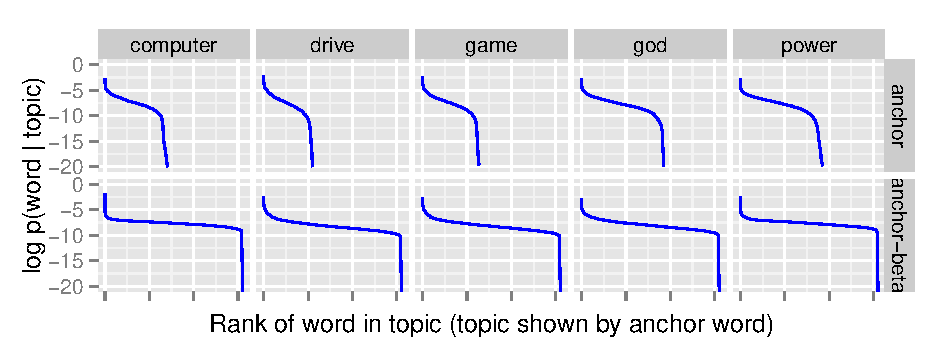
\includegraphics[width=\linewidth]{2015_naacl_qb_coref/auto_fig/density}
\end{center}
   \caption{Density of quiz bowl vs.\ \conll{} coreference both for raw and nested mentions.}
\label{fig:dense}
\end{figure}

A player's job is to
determine\footnote{In actual competition, it is a race to see which
  team can identify the coreference faster, but we ignore that aspect
  here.} the entity referenced by the question.  Each sentence contains
progressively more informative references and more well-known clues.  For
example, a question on Sherlock Holmes might refer to him as ``he'',
``this character'', ``this housemate of Dr. Watson'', and finally
``this detective and resident of 221B Baker Street''. While quiz bowl has been viewed as a classification
task~\cite{IyyerQA2014}, previous work has ignored the
fundamental task of coreference.  Nevertheless, quiz bowl data are dense and
diverse in coreference examples. For example, nested mentions, which are
difficult for both humans and machines, are very rare in the newswire text of
OntoNotes---0.25 mentions per sentence---while quiz bowl contains 1.16 mentions
per sentence (Figure~\ref{fig:dense}). Examples of nested mentions can be seen in
in Table~\ref{table1}. Since quiz bowl is a game, it makes the task of solving coreference interesting
and \emph{challenging} for an annotator. In the next section, we use the
intrinsic fun of this task to create a new annotated coreference dataset.

% \begin{figure}[ht]
% \begin{center}
% 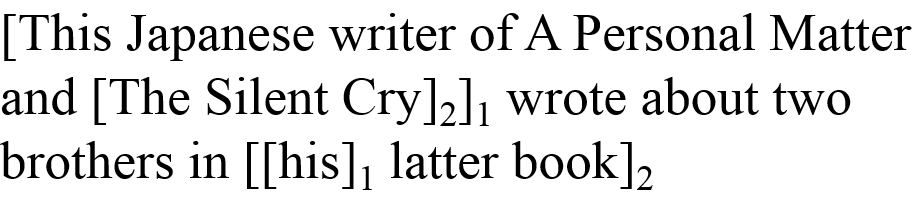
\includegraphics[scale = 0.25]{2015_naacl_qb_coref/figures/nested.png}
% \end{center}
%    \caption{Two coreference pairs, nested in each other}
%  \label{fig:nested}
% \end{figure}
